\section{Results}

\subsection{Sample-level alignment audit supports the core modelling table}

The alignment audit verified that each of the five cancer-internal modelling tables contained one labelled row per unique tumor sample, with no duplicate \texttt{sampleId} values and no patients contributing multiple labelled samples (Table~\ref{tab:alignment_audit}). All rows were primary solid tumor samples. The mismatch-core modalities were fully present at the sample level in UCEC, COADREAD, and HNSC, and nearly complete in KIRC (98.8\%) and PRAD (98.8\%). This audit establishes the aligned baseline from which simulated mismatch was introduced; the mismatch experiment therefore tests sensitivity to broken sample pairing rather than correcting a known duplicate-key problem in the original tables.

\begin{table}[ht]
\centering
\caption{Sample-level alignment audit for the five cancer-internal tasks. Core completeness refers to rows with at least one observed feature in mRNA, GISTIC copy number, methylation, and mutation. RPPA is shown as sample-level presence of any RPPA feature and is distinct from feature-level sparsity.}
\resizebox{\textwidth}{!}{%
\begin{tabular}{lrrrrrr}
\toprule
Task & Labelled rows & Unique samples & Duplicate samples & Unique patients & Multi-sample patients & Core-complete rows \\
\midrule
UCEC molecular subtype & 507 & 507 & 0 & 507 & 0 & 507 (100.0\%) \\
COADREAD molecular subtype & 449 & 449 & 0 & 449 & 0 & 449 (100.0\%) \\
HNSC HPV status & 487 & 487 & 0 & 487 & 0 & 487 (100.0\%) \\
KIRC grade & 504 & 504 & 0 & 504 & 0 & 498 (98.8\%) \\
PRAD pathologic T stage & 487 & 487 & 0 & 487 & 0 & 481 (98.8\%) \\
\bottomrule
\end{tabular}
}
\label{tab:alignment_audit}
\end{table}

\subsection{Modality coverage differs strongly across omics layers}

Core mRNA, copy-number, methylation, and mutation features had high observed fractions across the five TCGA cancer-internal tasks. In contrast, RPPA was sparse, with feature-level observed fractions ranging from 5.7\% in HNSC HPV status to 12.4\% in KIRC grade (Figure~\ref{fig:coverage}). This result supports treating modality coverage as a pre-modeling audit step rather than assuming that all nominally available omics layers should be fused.

\begin{figure}[ht]
\centering
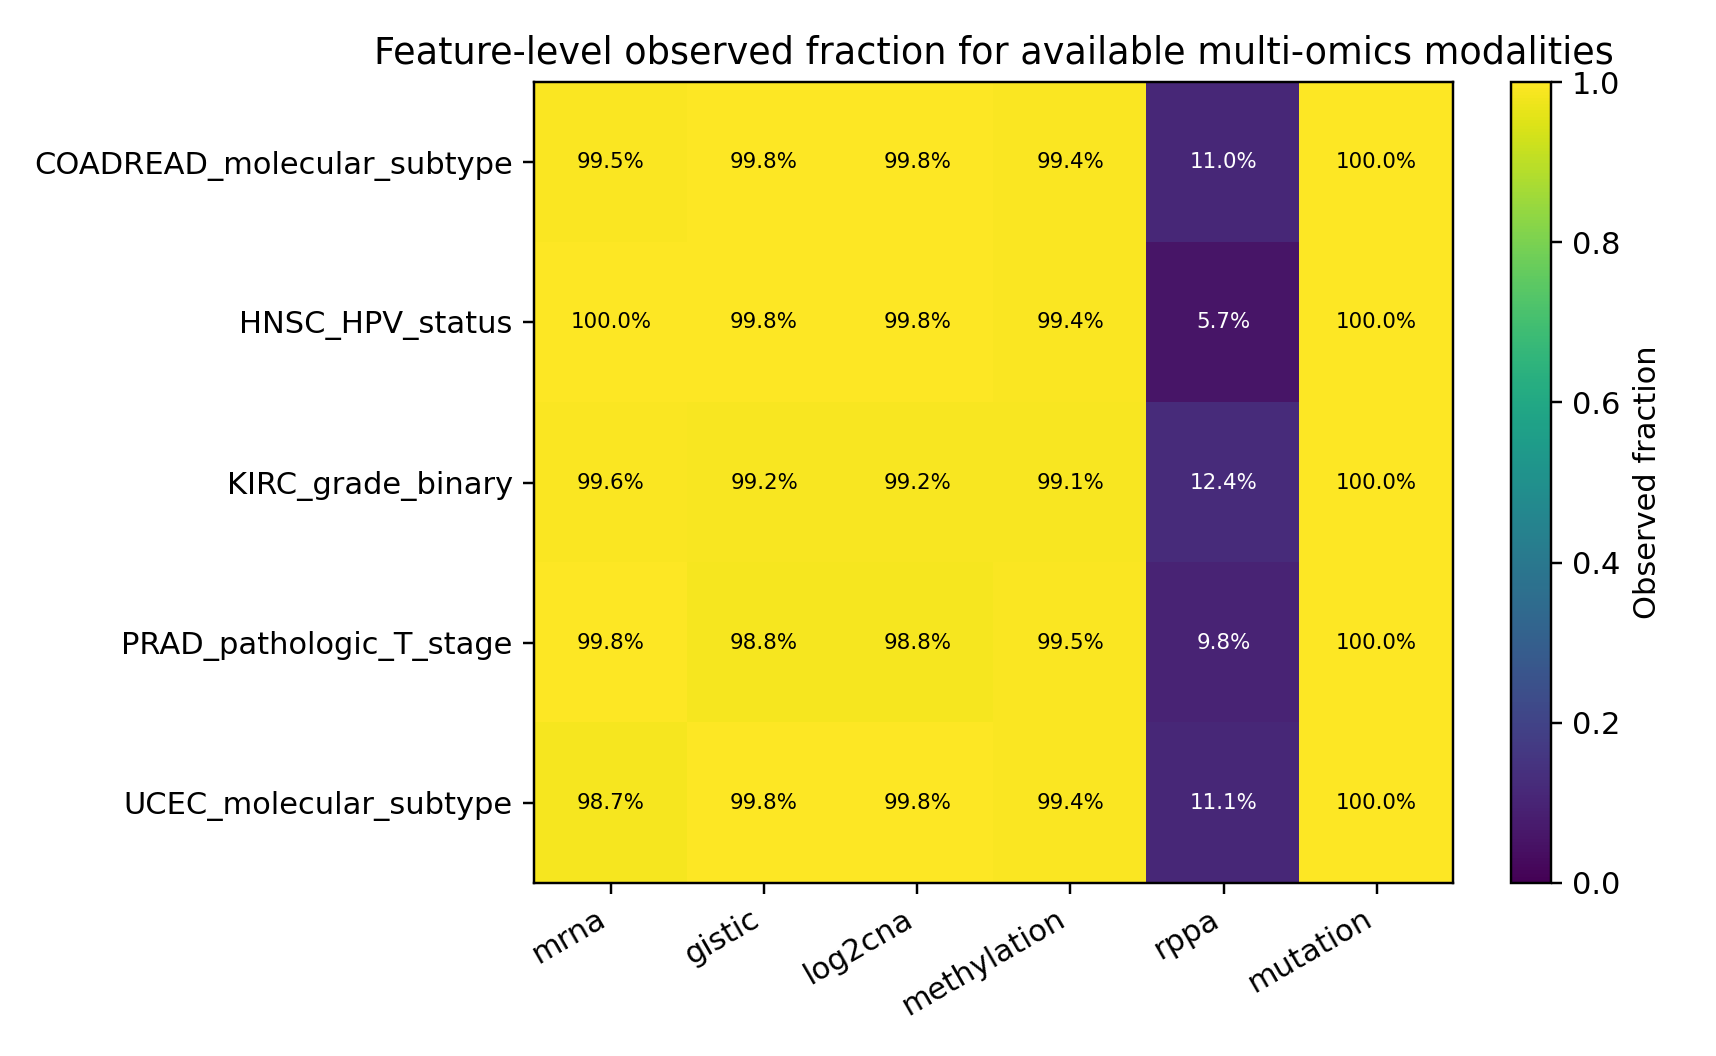
\includegraphics[width=\textwidth]{figures/modality_coverage_heatmap.png}
\caption{Feature-level observed fraction across available multi-omics modalities in five TCGA cancer-internal tasks. RPPA coverage was substantially lower than mRNA, copy-number, methylation, and mutation coverage.}
\label{fig:coverage}
\end{figure}

\subsection{The 10-cancer audit reveals broad assay heterogeneity}

At the full PanCancer level, mutation, copy-number, and methylation features had high observed fractions in most cancers, but coverage was not uniform across assays or cancer types. GBM had low observed mRNA feature coverage in the processed table (26\%), OV showed intermediate mRNA coverage (51\%), and RPPA remained sparse across all 10 cancer types (approximately 5\%--12\% observed feature fraction; Figure~\ref{fig:pancancer_coverage}). This broader audit confirms that modality coverage is not merely a task-specific concern: it is a recurring property of public multi-omics resources.

\begin{figure}[ht]
\centering
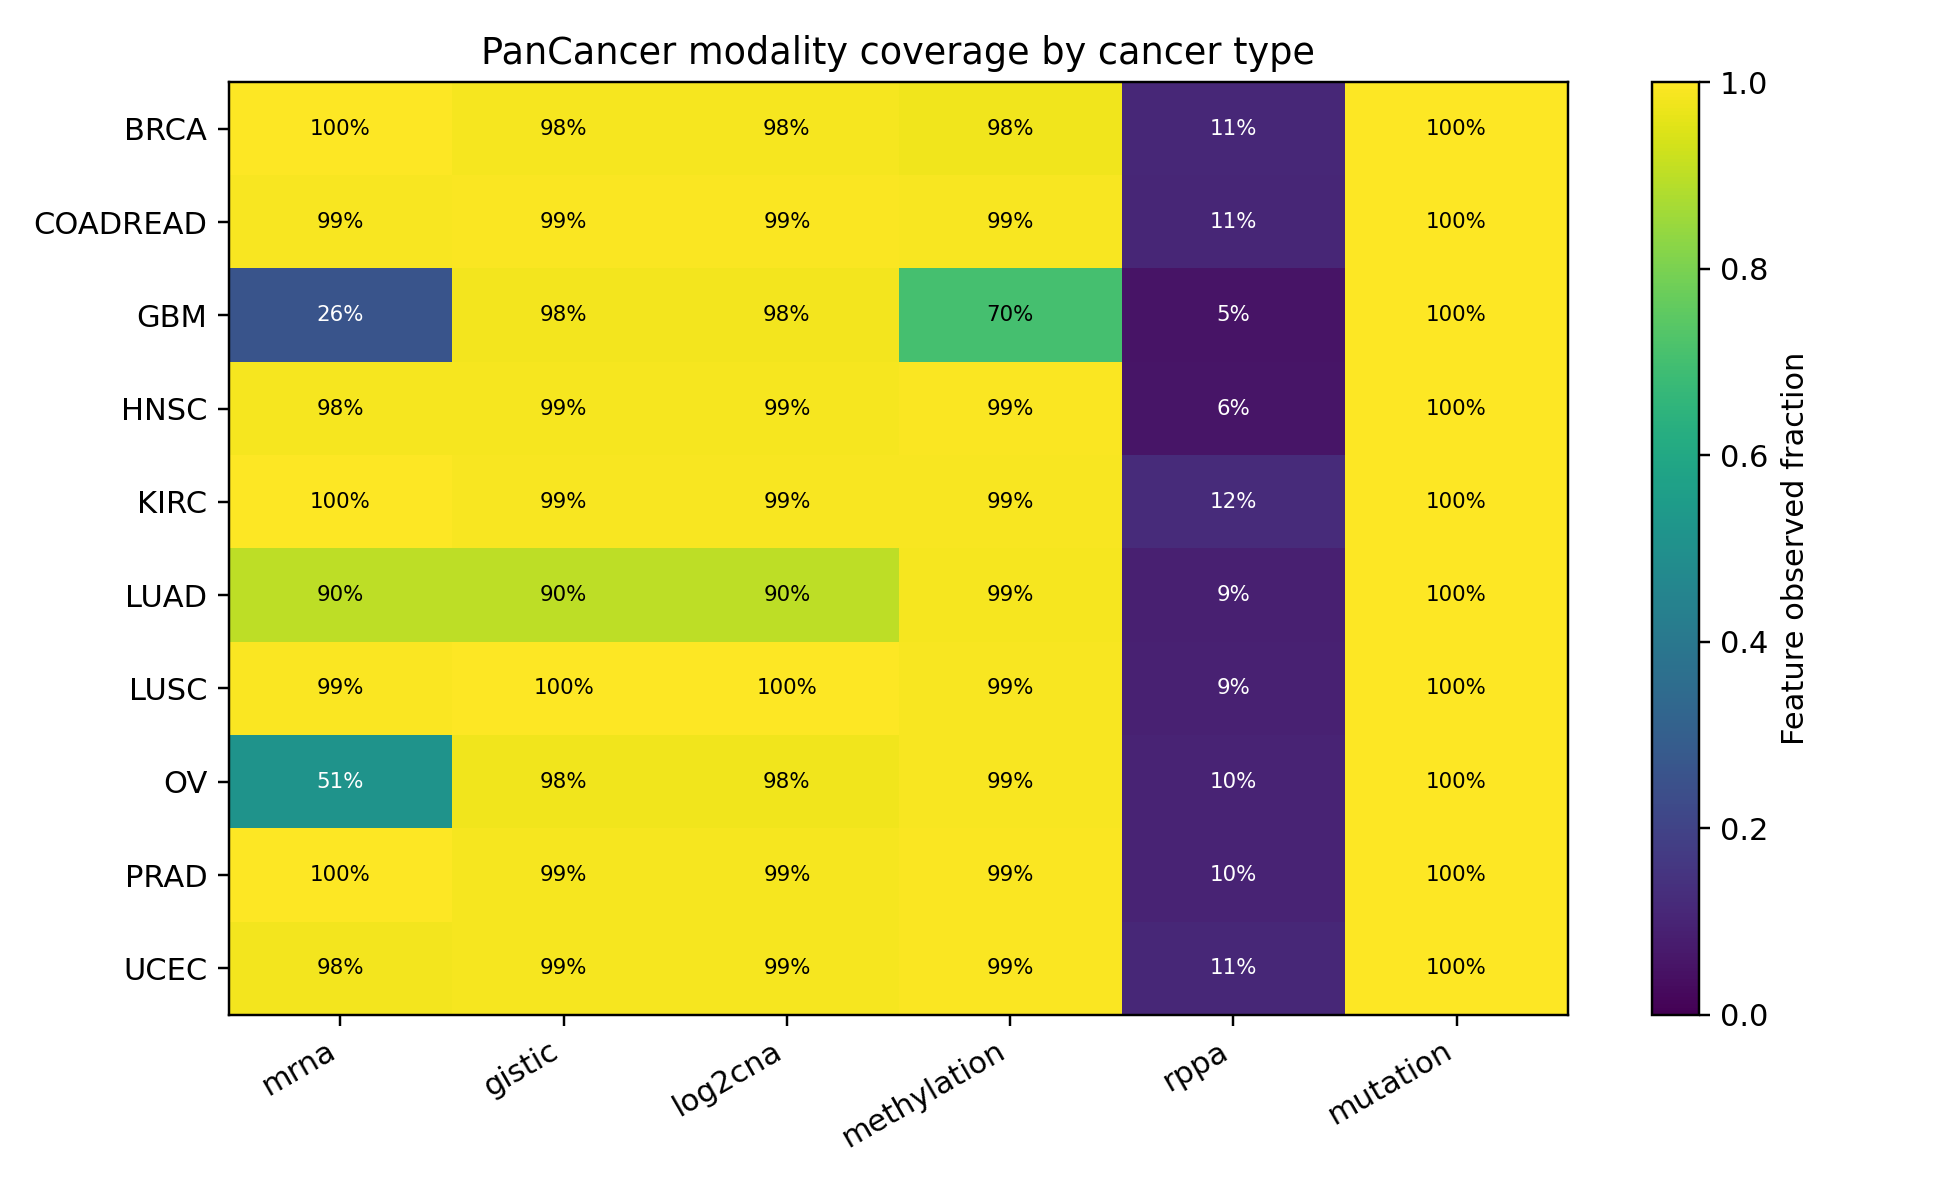
\includegraphics[width=\textwidth]{figures/pancancer_modality_coverage_by_cancer.png}
\caption{PanCancer modality coverage by cancer type. Values show the feature-level observed fraction for each assay block in the 10-cancer TCGA PanCancer table. RPPA was consistently sparse, and some cancers also showed reduced mRNA coverage in the processed feature table.}
\label{fig:pancancer_coverage}
\end{figure}

\subsection{Exploratory endpoint discovery broadens the task landscape}

Across the 10 TCGA PanCancer cohorts, the exploratory clinical endpoint screen identified 21 candidate within-cancer tasks with sufficient class support (Figure~\ref{fig:expanded_scope_availability}). These included four grade tasks, four molecular or histologic subtype tasks, six early- versus advanced-stage tasks, and seven pathologic T-stage tasks. The available task count differed by cancer type: BRCA, COADREAD, HNSC, KIRC, UCEC, LUAD, LUSC, OV, and PRAD each contributed at least one clinically interpretable endpoint, whereas GBM did not meet the predefined endpoint and class-count criteria in this screen.

\begin{figure}[ht]
\centering
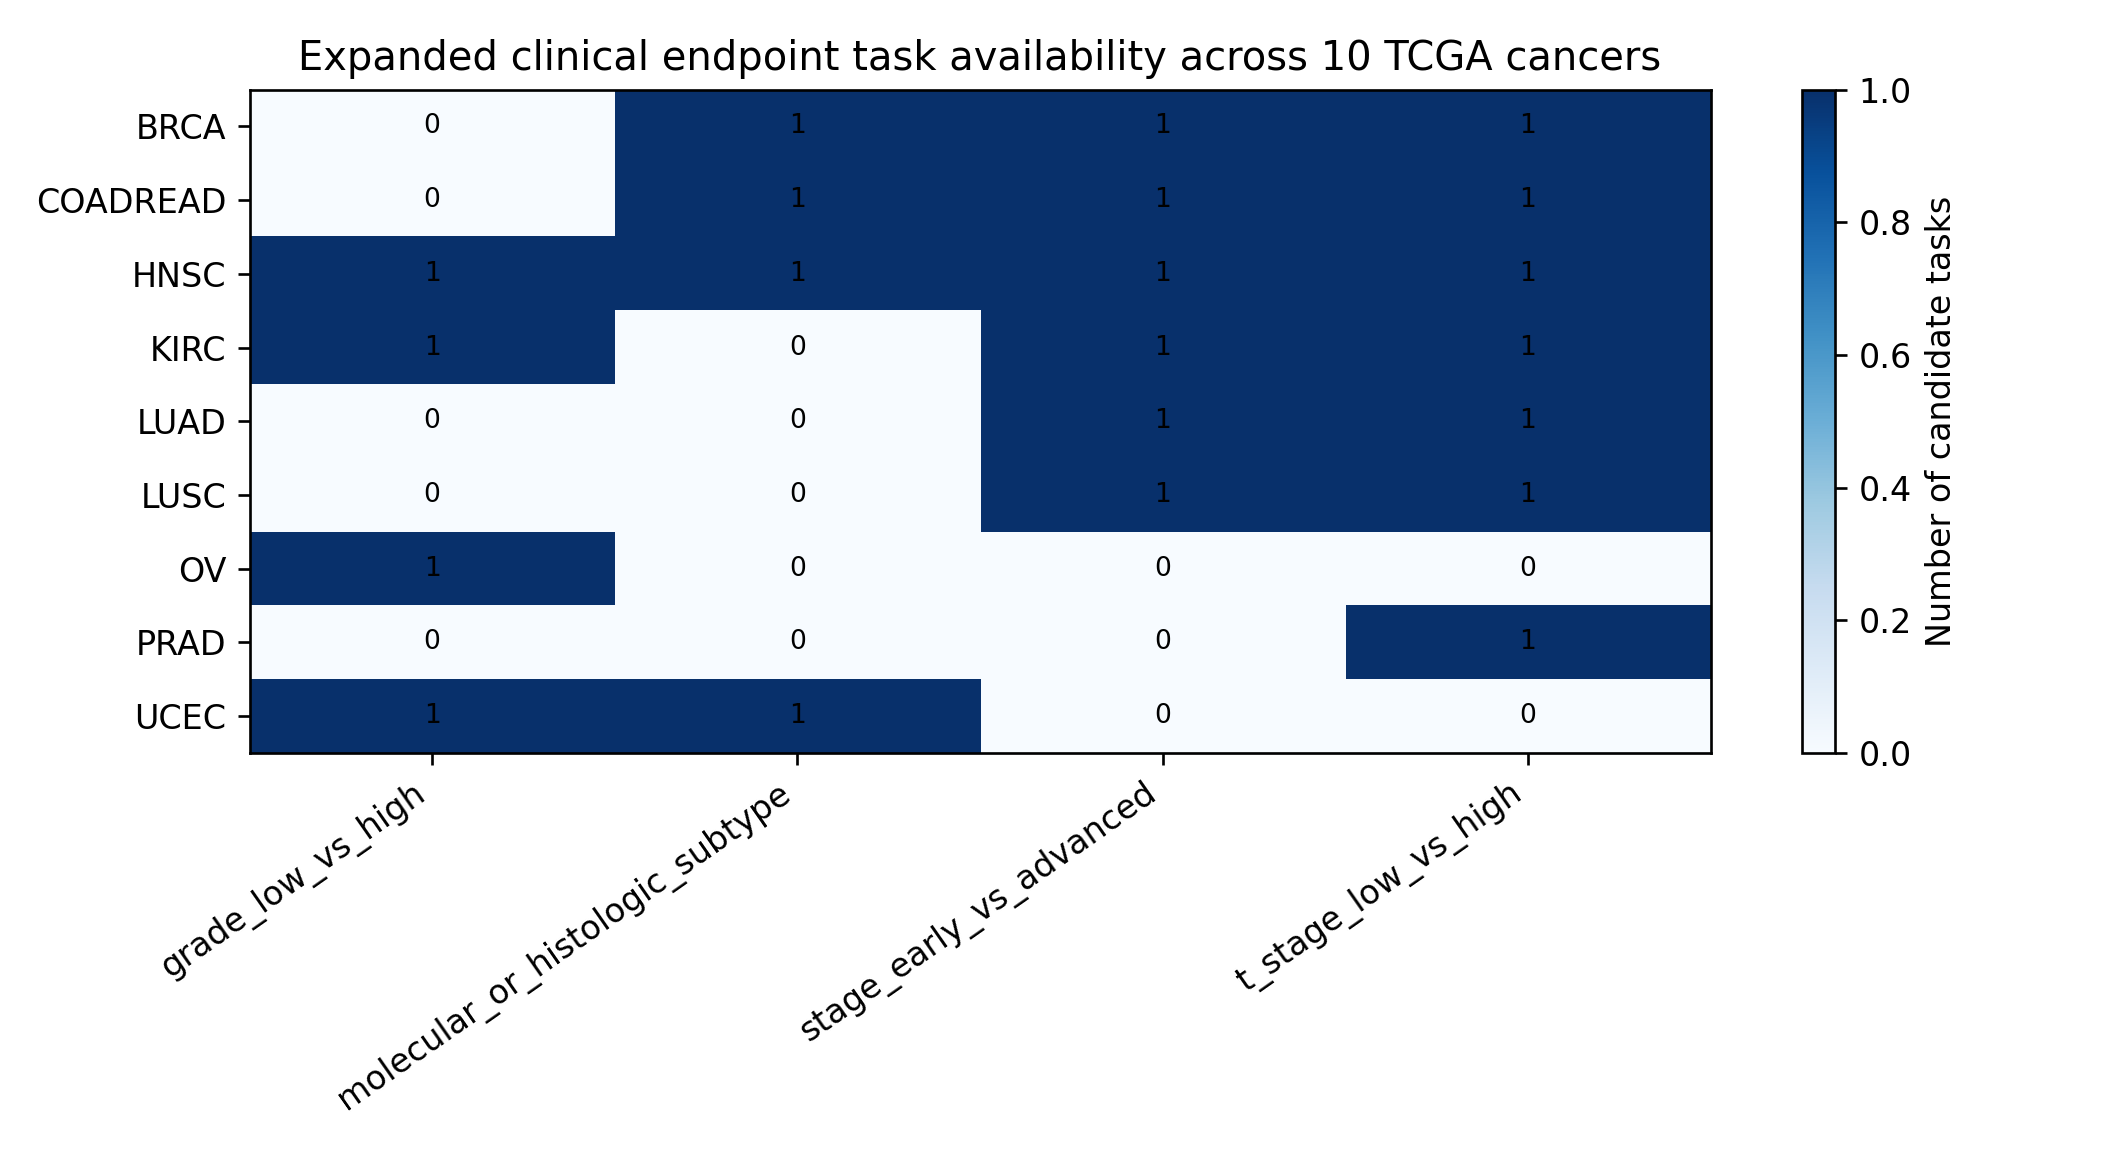
\includegraphics[width=0.90\textwidth]{figures/expanded_scope_task_availability.png}
\caption{Expanded within-cancer endpoint availability across the 10 TCGA PanCancer cohorts. Candidate tasks were retained only when labels could be harmonized into a clinically interpretable endpoint and each retained class had at least 40 labelled samples.}
\label{fig:expanded_scope_availability}
\end{figure}

The lightweight three-fold baseline screen showed substantial variation in endpoint difficulty (Figure~\ref{fig:expanded_scope_f1}; Table~\ref{tab:expanded_scope}). Molecular or histologic subtype tasks were the most learnable group, with best-task macro F1 values ranging from 0.8178 to 0.9387. Grade prediction was heterogeneous, ranging from 0.5582 in OV to 0.8341 in UCEC. Stage and pathologic T-stage tasks were generally harder, with best-task macro F1 ranges of 0.5152--0.6893 and 0.5050--0.7049, respectively. These results expand the benchmark from a small set of hand-curated endpoints to a broader map of candidate task availability and difficulty while preserving the main manuscript's focus on alignment, mismatch sensitivity, and cohort shift.

\begin{figure}[ht]
\centering
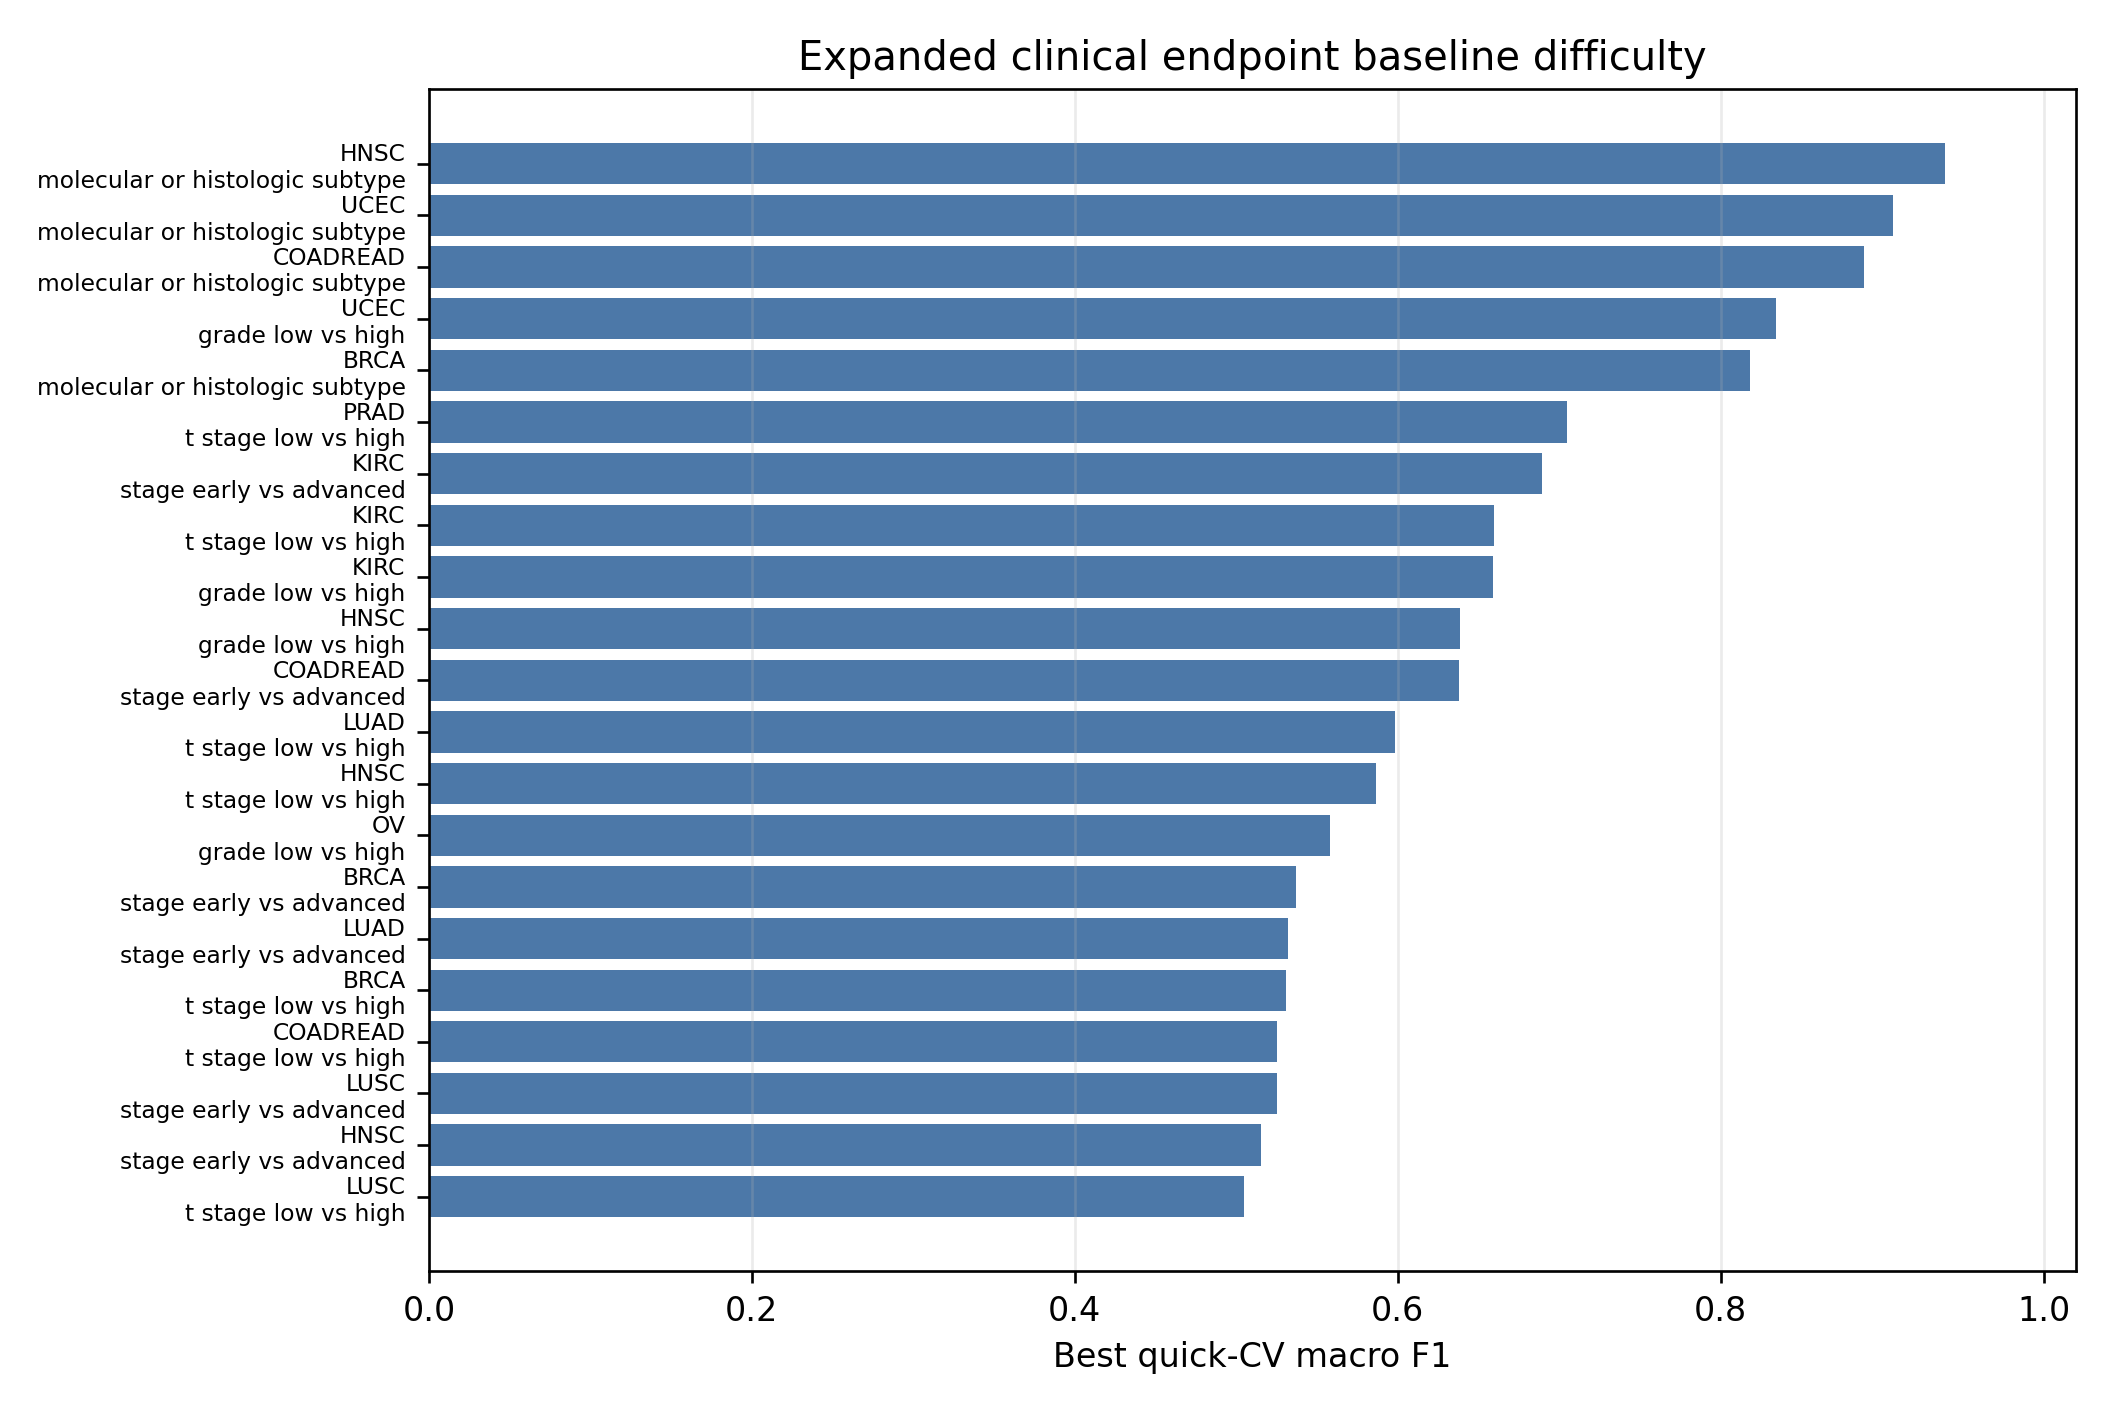
\includegraphics[width=\textwidth]{figures/expanded_scope_endpoint_f1.png}
\caption{Quick baseline difficulty screen for expanded within-cancer endpoints. Values show the better macro F1 of elastic-net logistic regression and ExtraTrees under three-fold cross-validation with training-fold feature selection.}
\label{fig:expanded_scope_f1}
\end{figure}

\begin{table}[ht]
\centering
\caption{Expanded endpoint families discovered across the 10-cancer TCGA PanCancer clinical screen. Macro F1 ranges use the better of elastic-net logistic regression and ExtraTrees for each task in the lightweight three-fold screen.}
\label{tab:expanded_scope}
\resizebox{\textwidth}{!}{%
\begin{tabular}{lrrrl}
\toprule
Endpoint family & Candidate tasks & Cancers represented & Best macro F1 range & Highest-scoring task \\
\midrule
Grade low vs high & 4 & 4 & 0.5582--0.8341 & UCEC grade \\
Molecular or histologic subtype & 4 & 4 & 0.8178--0.9387 & HNSC subtype \\
Stage early vs advanced & 6 & 6 & 0.5152--0.6893 & KIRC stage \\
Pathologic T stage low vs high & 7 & 7 & 0.5050--0.7049 & PRAD pathologic T stage \\
\bottomrule
\end{tabular}
}
\end{table}

\subsection{Simulated sample mismatch reduces multi-omics prediction performance}

When non-mRNA omics layers were permuted across samples, multi-omics performance declined in a task- and model-dependent manner (Figure~\ref{fig:mismatch}). The largest aligned-to-fully-misaligned macro F1 drops occurred for COADREAD molecular subtype using ExtraTrees (0.8893 to 0.5008; drop 0.3885) and UCEC molecular subtype using ExtraTrees (0.9141 to 0.5914; drop 0.3227). Logistic regression was less sensitive in COADREAD but still showed a notable UCEC drop (0.9088 to 0.6943; drop 0.2145). KIRC grade and PRAD pathologic T stage showed smaller drops, suggesting that some tasks were driven mainly by mRNA or by robust single-modality signals.

\begin{figure}[ht]
\centering
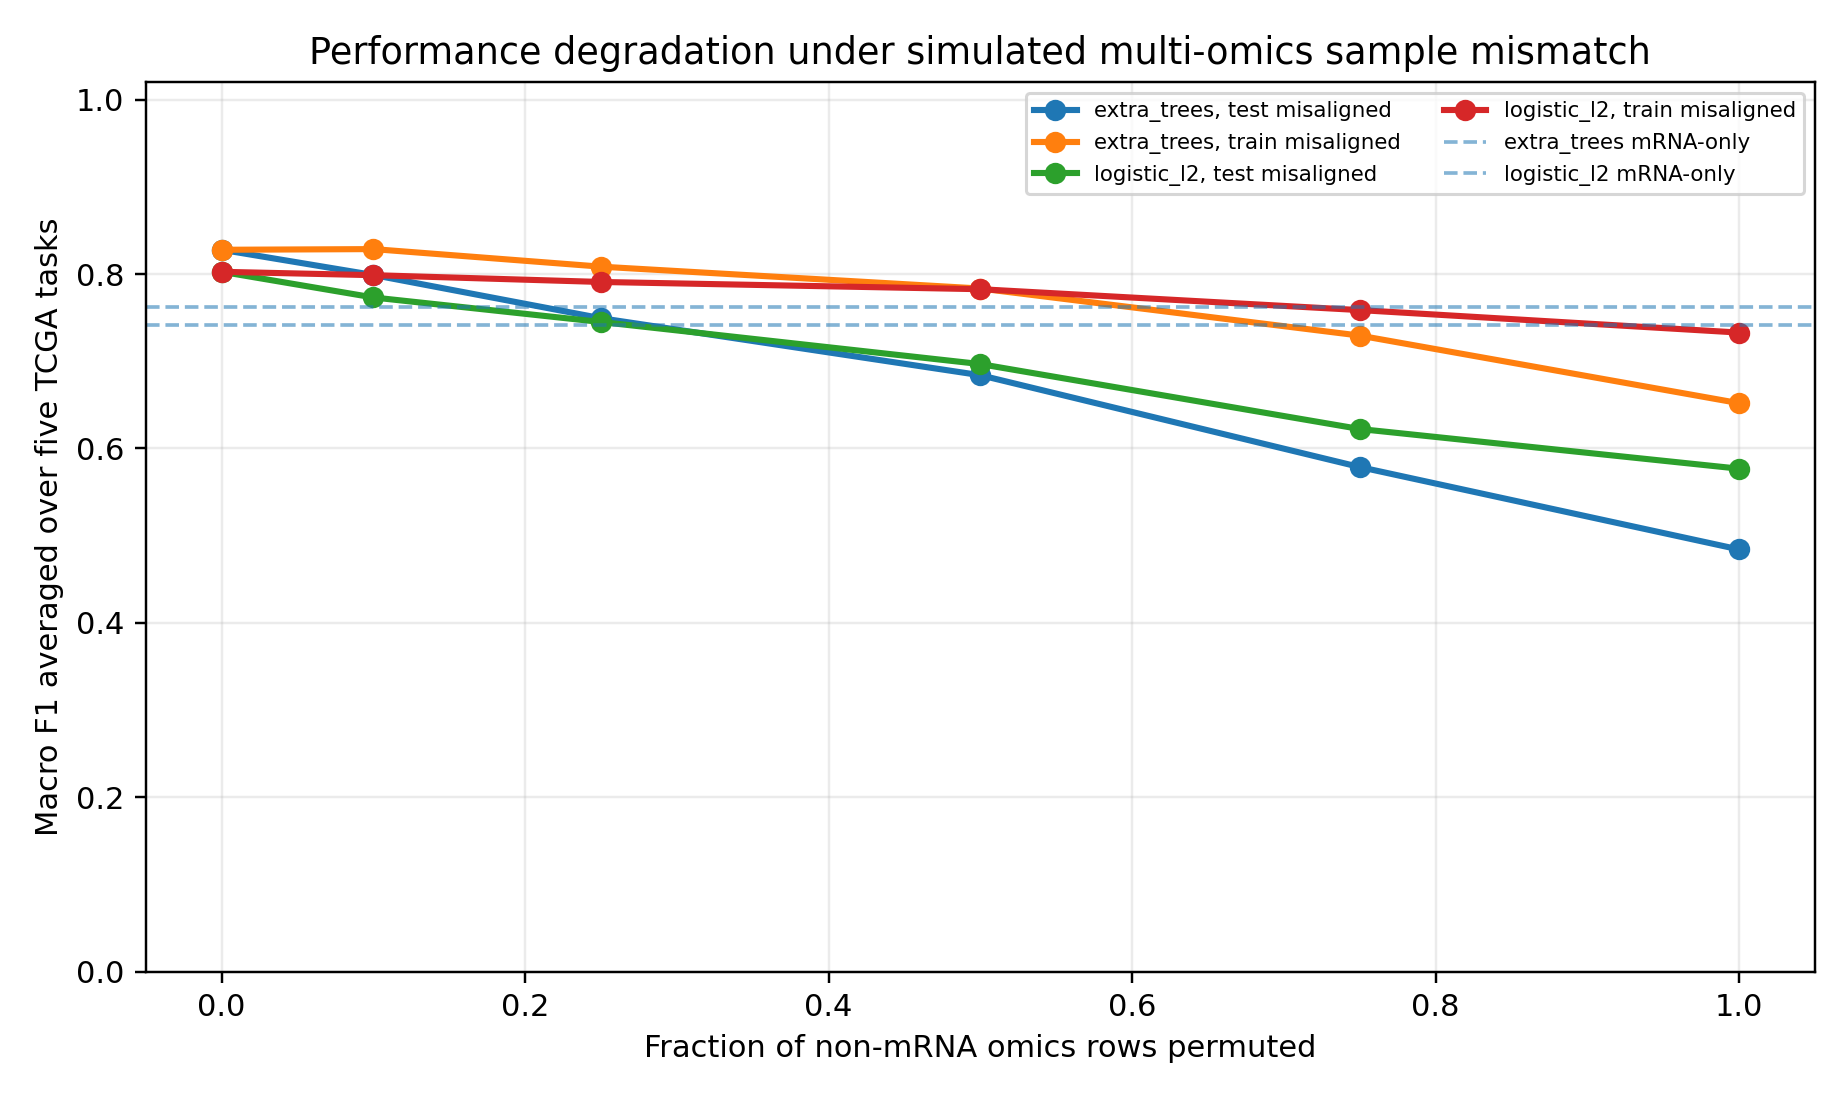
\includegraphics[width=\textwidth]{figures/misalignment_degradation.png}
\caption{Macro F1 degradation under simulated sample mismatch. Non-mRNA omics rows were permuted at increasing rates while preserving each modality's marginal distribution. Lines summarize mean macro F1 across the five TCGA cancer-internal tasks and three random seeds. Dashed lines indicate mRNA-only reference performance.}
\label{fig:mismatch}
\end{figure}

\begin{table}[ht]
\centering
\caption{Aligned versus fully misaligned training data in the cancer-internal stress test.}
\resizebox{\textwidth}{!}{%
\begin{tabular}{llrrr}
\toprule
Task & Model & Aligned macro F1 & Fully misaligned macro F1 & Drop \\
\midrule
COADREAD molecular subtype & ExtraTrees & 0.8893 & 0.5008 & 0.3885 \\
UCEC molecular subtype & ExtraTrees & 0.9141 & 0.5914 & 0.3227 \\
UCEC molecular subtype & Logistic L2 & 0.9088 & 0.6943 & 0.2145 \\
HNSC HPV status & ExtraTrees & 0.9573 & 0.8405 & 0.1168 \\
HNSC HPV status & Logistic L2 & 0.9640 & 0.9201 & 0.0439 \\
COADREAD molecular subtype & Logistic L2 & 0.8686 & 0.8323 & 0.0363 \\
KIRC grade & ExtraTrees & 0.7200 & 0.6868 & 0.0332 \\
KIRC grade & Logistic L2 & 0.6498 & 0.6206 & 0.0292 \\
PRAD pathologic T stage & Logistic L2 & 0.6215 & 0.5970 & 0.0245 \\
PRAD pathologic T stage & ExtraTrees & 0.6583 & 0.6400 & 0.0183 \\
\bottomrule
\end{tabular}
}
\label{tab:mismatch}
\end{table}

The Liquid-family mismatch extension showed the same qualitative pattern: Liquid/CfC and small-Liquid/CfC were not immune to sample-level pairing errors (Figure~\ref{fig:liquid_mismatch}). Under fully mismatched training data, the largest Liquid-family macro F1 drops occurred for COADREAD small-Liquid/CfC (0.8041 to 0.5639; drop 0.2402), UCEC Liquid/CfC (0.8982 to 0.6587; drop 0.2396), and UCEC small-Liquid/CfC (0.8487 to 0.6257; drop 0.2230). HNSC also showed drops above 0.11 for both Liquid variants, whereas KIRC and PRAD were less sensitive, particularly for full Liquid/CfC.

\begin{figure}[ht]
\centering
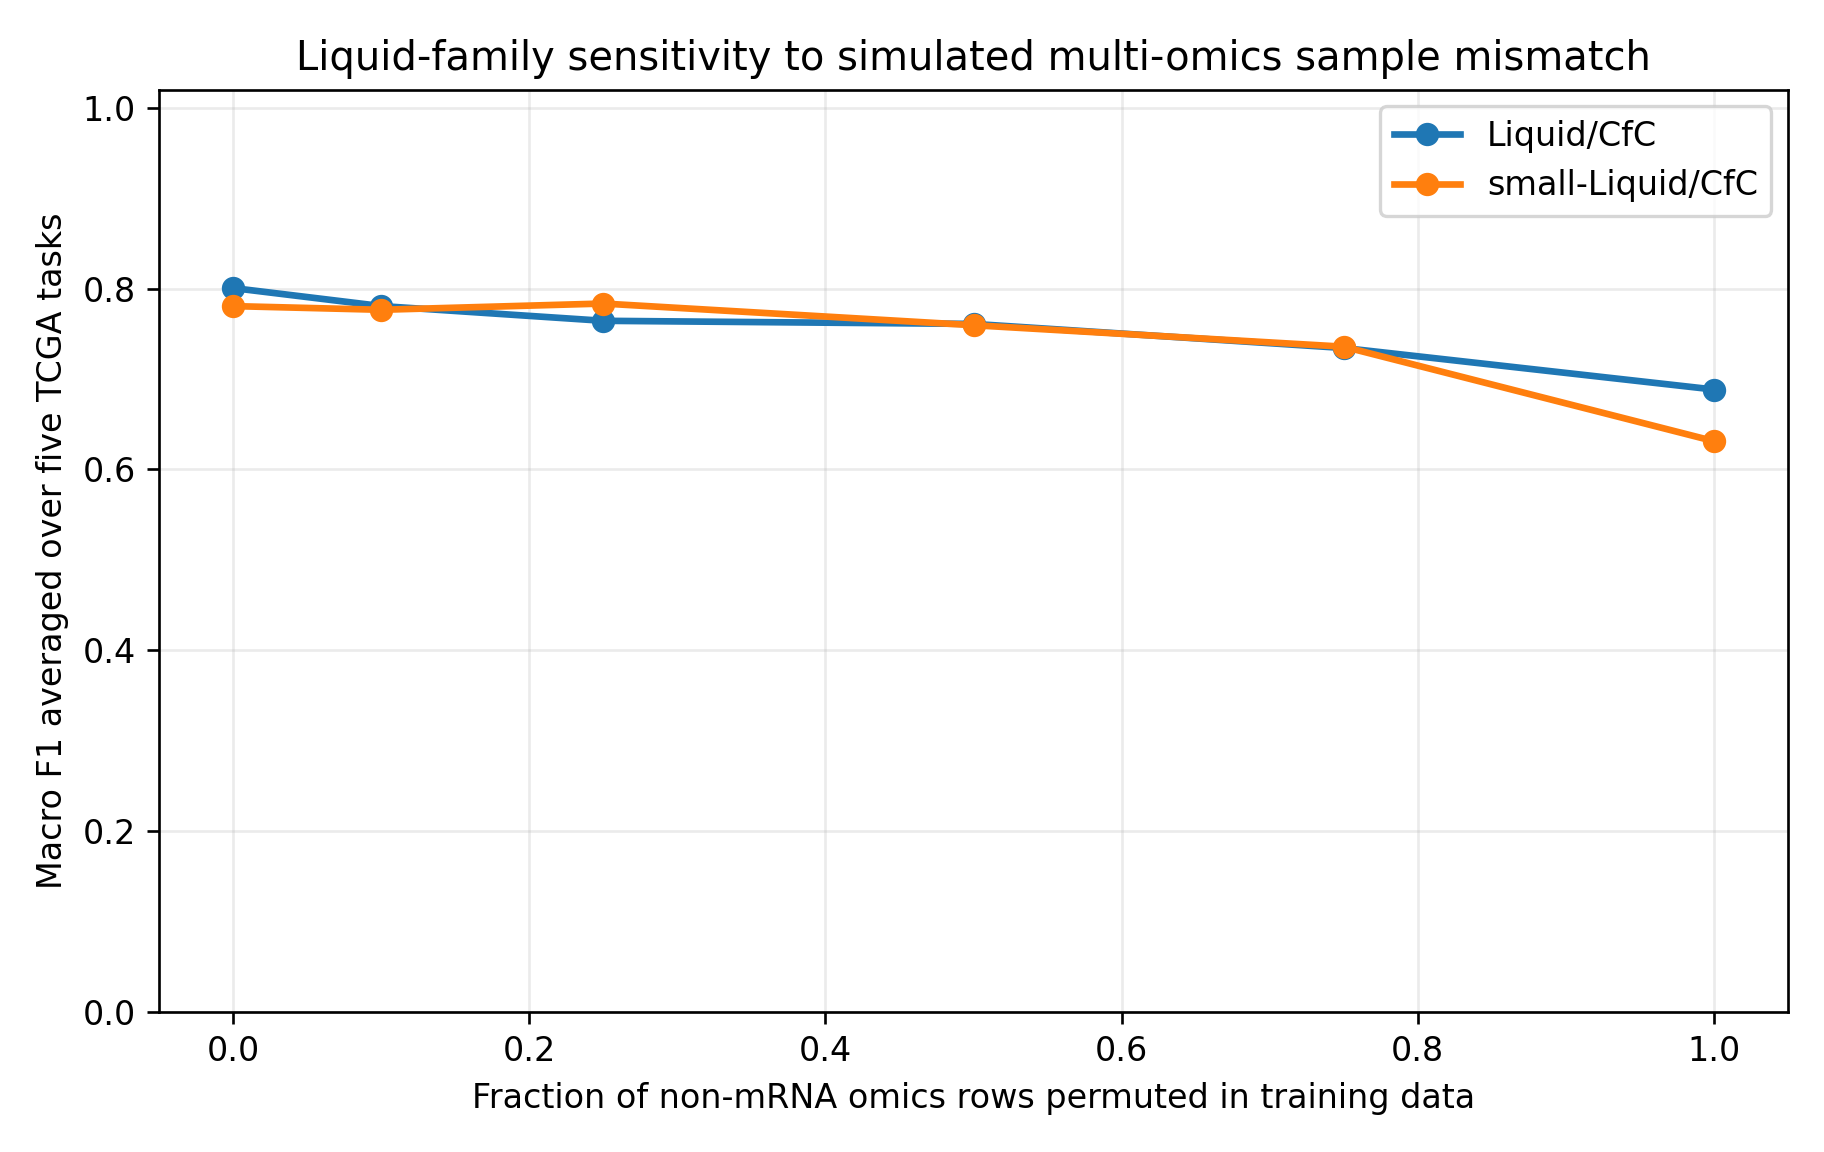
\includegraphics[width=0.86\textwidth]{figures/liquid_mismatch_degradation.png}
\caption{Liquid-family sensitivity to simulated multi-omics sample mismatch. Lines show mean macro F1 across the five TCGA cancer-internal tasks and three random seeds when non-mRNA omics rows were permuted in the training data.}
\label{fig:liquid_mismatch}
\end{figure}

\begin{table}[ht]
\centering
\caption{Liquid-family aligned versus fully misaligned training data in the cancer-internal stress test.}
\resizebox{\textwidth}{!}{%
\begin{tabular}{llrrr}
\toprule
Task & Model & Aligned macro F1 & Fully misaligned macro F1 & Drop \\
\midrule
COADREAD molecular subtype & small-Liquid/CfC & 0.8041 & 0.5639 & 0.2402 \\
UCEC molecular subtype & Liquid/CfC & 0.8982 & 0.6587 & 0.2396 \\
UCEC molecular subtype & small-Liquid/CfC & 0.8487 & 0.6257 & 0.2230 \\
COADREAD molecular subtype & Liquid/CfC & 0.8382 & 0.7010 & 0.1372 \\
HNSC HPV status & small-Liquid/CfC & 0.9236 & 0.7996 & 0.1240 \\
HNSC HPV status & Liquid/CfC & 0.9445 & 0.8259 & 0.1187 \\
PRAD pathologic T stage & small-Liquid/CfC & 0.6667 & 0.5714 & 0.0953 \\
KIRC grade & small-Liquid/CfC & 0.6601 & 0.5959 & 0.0642 \\
PRAD pathologic T stage & Liquid/CfC & 0.6690 & 0.6247 & 0.0443 \\
KIRC grade & Liquid/CfC & 0.6529 & 0.6317 & 0.0212 \\
\bottomrule
\end{tabular}
}
\label{tab:liquid_mismatch}
\end{table}

\subsection{Expanded baselines do not support a universal architecture winner}

The expanded 10-fold benchmark included seven model families across the five cancer-internal tasks (Figure~\ref{fig:expanded_baseline}). The leading model differed by task: ExtraTrees achieved the highest mean macro F1 for COADREAD molecular subtype (0.8676) and UCEC molecular subtype (0.8944), elastic-net logistic regression led HNSC HPV status (0.9469), and Random Forest led KIRC grade (0.6784) and PRAD pathologic T stage (0.6839). Liquid/CfC and small-Liquid/CfC were competitive in several tasks but were not consistently superior.

\begin{figure}[ht]
\centering
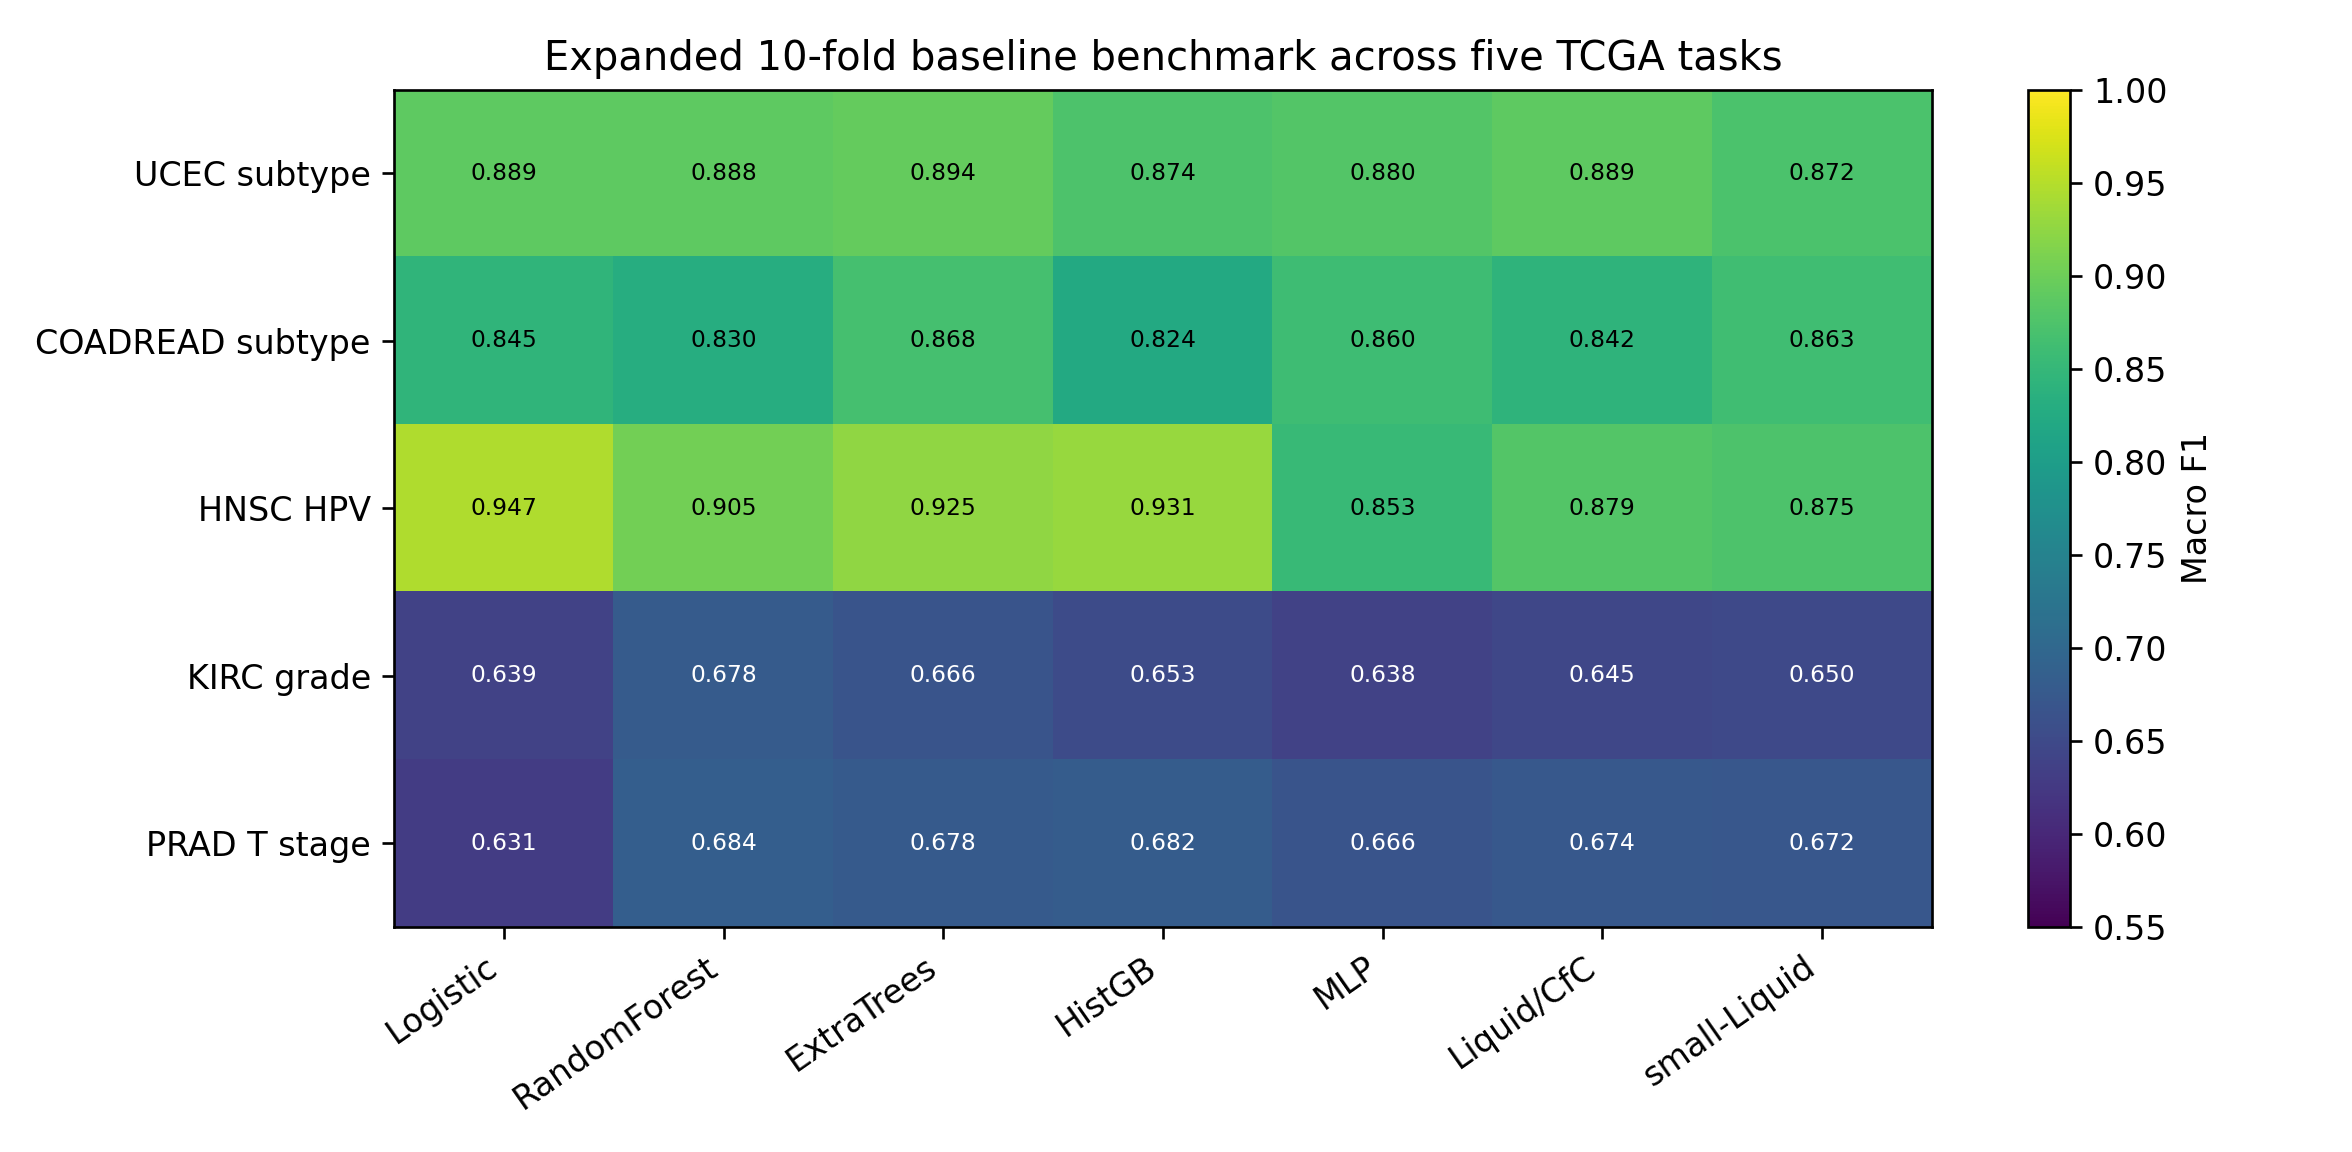
\includegraphics[width=\textwidth]{figures/expanded_baseline_cv_heatmap.png}
\caption{Expanded 10-fold baseline benchmark across five TCGA cancer-internal tasks. Values show mean macro F1 for each model family. The leading architecture differed by task, and no single model family dominated all endpoints.}
\label{fig:expanded_baseline}
\end{figure}

\begin{table}[ht]
\centering
\caption{Best 10-fold baseline model per cancer-internal task and exploratory paired top-versus-runner-up fold-level comparison.}
\resizebox{\textwidth}{!}{%
\begin{tabular}{lllrrrr}
\toprule
Task & Top model & Runner-up & Top macro F1 & Mean F1 diff & 95\% CI for diff & Exploratory Holm \(p\) \\
\midrule
COADREAD molecular subtype & ExtraTrees & small-Liquid/CfC & 0.8676 & 0.0048 & [-0.0431, 0.0514] & 1.0000 \\
HNSC HPV status & Elastic-net logistic & HistGradientBoosting & 0.9469 & 0.0159 & [-0.0141, 0.0470] & 1.0000 \\
KIRC grade & Random Forest & ExtraTrees & 0.6784 & 0.0122 & [-0.0057, 0.0310] & 1.0000 \\
PRAD pathologic T stage & Random Forest & HistGradientBoosting & 0.6839 & 0.0021 & [-0.0451, 0.0389] & 1.0000 \\
UCEC molecular subtype & ExtraTrees & Elastic-net logistic & 0.8944 & 0.0053 & [-0.0391, 0.0471] & 1.0000 \\
\bottomrule
\end{tabular}
}
\label{tab:expanded_baseline}
\end{table}

Exploratory fold-level paired comparisons reinforced the effect-size interpretation. All top-versus-runner-up confidence intervals crossed zero (Table~\ref{tab:expanded_baseline}). In the broader top-versus-all diagnostics, the clearest contrast was HNSC HPV status, where elastic-net logistic regression exceeded MLP by 0.0939 macro F1 (95\% CI 0.0444--0.1382; exploratory adjusted \(p=0.0469\)). Because CV folds are not independent biological samples, these \(p\) values were not treated as definitive inferential tests. The benchmark therefore supports a task- and data-dependent reliability interpretation rather than a claim that Liquid/CfC or any other architecture is universally best.

\subsection{Liquid/CfC serves as a task-dependent neural comparator}

The expanded benchmark also allowed us to examine where Liquid/CfC-style models were relatively strong or weak (Table~\ref{tab:liquid_applicability}). Liquid/CfC or small-Liquid/CfC was near the best model in COADREAD molecular subtype, UCEC molecular subtype, and PRAD pathologic T stage, with mean macro F1 within 0.01 of the task-leading model. However, Liquid/CfC was weaker in HNSC HPV status, where elastic-net logistic regression led by 0.0675 macro F1 over Liquid/CfC and 0.0722 over small-Liquid/CfC. In KIRC grade, Random Forest also led the Liquid variants by approximately 0.03 macro F1.

\begin{table}[ht]
\centering
\caption{Task-level interpretation of Liquid/CfC and small-Liquid/CfC performance. Delta values are relative to the best 10-fold mean macro F1 model for each task.}
\resizebox{\textwidth}{!}{%
\begin{tabular}{llrrl}
\toprule
Task & Best Liquid-family model & Rank & Delta versus best & Interpretation \\
\midrule
COADREAD molecular subtype & small-Liquid/CfC & 2 & -0.0048 & Near-best; competitive with ExtraTrees \\
UCEC molecular subtype & Liquid/CfC & 3 & -0.0059 & Near-best; no clear gap to ExtraTrees \\
PRAD pathologic T stage & Liquid/CfC & 4 & -0.0097 & Near-best, but all models were close \\
KIRC grade & small-Liquid/CfC & 4 & -0.0283 & Modestly weaker than Random Forest \\
HNSC HPV status & Liquid/CfC & 5 & -0.0675 & Weaker than elastic-net logistic regression \\
\bottomrule
\end{tabular}
}
\label{tab:liquid_applicability}
\end{table}

These findings suggest a practical boundary for using Liquid/CfC in static cancer multi-omics. Liquid-style models may be useful when the task benefits from structured cross-modality integration and when no single sparse linear signal dominates. They appear less advantageous when the endpoint is already well separated by simpler feature combinations, as in HNSC HPV status, or when tabular tree ensembles capture the relevant nonlinearities with fewer modeling assumptions, as in KIRC grade. Thus, Liquid/CfC should be treated as a comparator whose value is task-dependent rather than as a default superior architecture for cancer multi-omics tables.

\subsection{Medical interpretation links model behavior to endpoint biology}

The task-level model patterns were medically interpretable rather than arbitrary (Table~\ref{tab:medical_interpretation}). UCEC and COADREAD molecular subtypes are defined by multiple biological mechanisms, including copy-number burden, microsatellite instability, polymerase-epsilon proofreading mutations, and epigenetic or expression programs. These endpoints are plausible settings for cross-modality integration, and Liquid-family models were near-best or strongly mismatch-sensitive in both tasks. HNSC HPV status, in contrast, is a high-signal viral-oncogenesis endpoint; the strongest model was elastic-net logistic regression, suggesting that simpler expression-associated decision boundaries can be sufficient. KIRC grade and PRAD pathologic T stage are partly histopathologic or anatomic endpoints, which may explain their lower molecular predictability and the potential value of future pathology or imaging-augmented extensions.

\begin{table}[ht]
\centering
\caption{Medical interpretation of the five cancer-internal endpoints and observed model behavior.}
\begingroup
\scriptsize
\setlength{\tabcolsep}{3pt}
\begin{tabular}{>{\raggedright\arraybackslash}p{0.14\textwidth}>{\raggedright\arraybackslash}p{0.26\textwidth}>{\raggedright\arraybackslash}p{0.26\textwidth}>{\raggedright\arraybackslash}p{0.24\textwidth}}
\toprule
Task & Endpoint biology & Why multi-omics may matter & Model interpretation \\
\midrule
UCEC molecular subtype & CN-high, CN-low, MSI, and POLE subtypes reflect copy-number burden, mismatch repair deficiency, and polymerase proofreading mutations. & CNA, mutation, methylation, and expression can provide complementary subtype signals. & Liquid/CfC was near-best and mismatch-sensitive, consistent with cross-modality relevance. \\
COADREAD molecular subtype & CIN, MSI, and genome-stable colorectal cancer reflect chromosomal instability, microsatellite instability, and epigenetic/expression programs. & The endpoint combines genome instability and transcriptomic or methylation programs. & small-Liquid/CfC was near-best, although ExtraTrees had the top mean macro F1. \\
HNSC HPV status & HPV-positive disease reflects viral oncogenesis and strong transcriptional/cell-cycle signatures. & Expression signal may already separate the endpoint strongly. & Elastic-net logistic regression was strongest; Liquid/CfC was not advantageous. \\
KIRC grade & Histologic grade reflects tumor aggressiveness, hypoxia/angiogenesis, chromatin remodeling, and VHL-related biology. & Bulk molecular features may only partly capture a histopathologic phenotype. & Random Forest was strongest; pathology imaging may be a natural complementary modality. \\
PRAD pathologic T stage & T stage reflects local invasion and anatomic extension, not a purely molecular phenotype. & Molecular signal is expected to be modest and may need clinical or imaging context. & Liquid/CfC was near-best, but all models were close. \\
\bottomrule
\end{tabular}
\endgroup
\label{tab:medical_interpretation}
\end{table}

\subsection{Cancer-type classification is much easier than within-cancer endpoint prediction}

The existing PanCancer cancer-type benchmark achieved a best macro F1 of 0.9904 across 10 cancer types. In one-vs-rest analyses using mRNA features alone, every cancer type was highly separable from the remaining cancers, with AUC values ranging from 0.9721 for OV to 0.9997 for COADREAD (Figure~\ref{fig:cancer_sep}). By contrast, the five clinically or molecularly meaningful within-cancer tasks were more variable: HNSC HPV status reached 0.9505 macro F1, UCEC and COADREAD molecular subtypes were near 0.91, while PRAD pathologic T stage and KIRC grade were near 0.70 (Figure~\ref{fig:task_difficulty}). This contrast is important because a high pan-cancer cancer-type score can mostly reflect strong tissue-of-origin structure, whereas clinically useful within-cancer prediction remains harder.

\begin{figure}[ht]
\centering
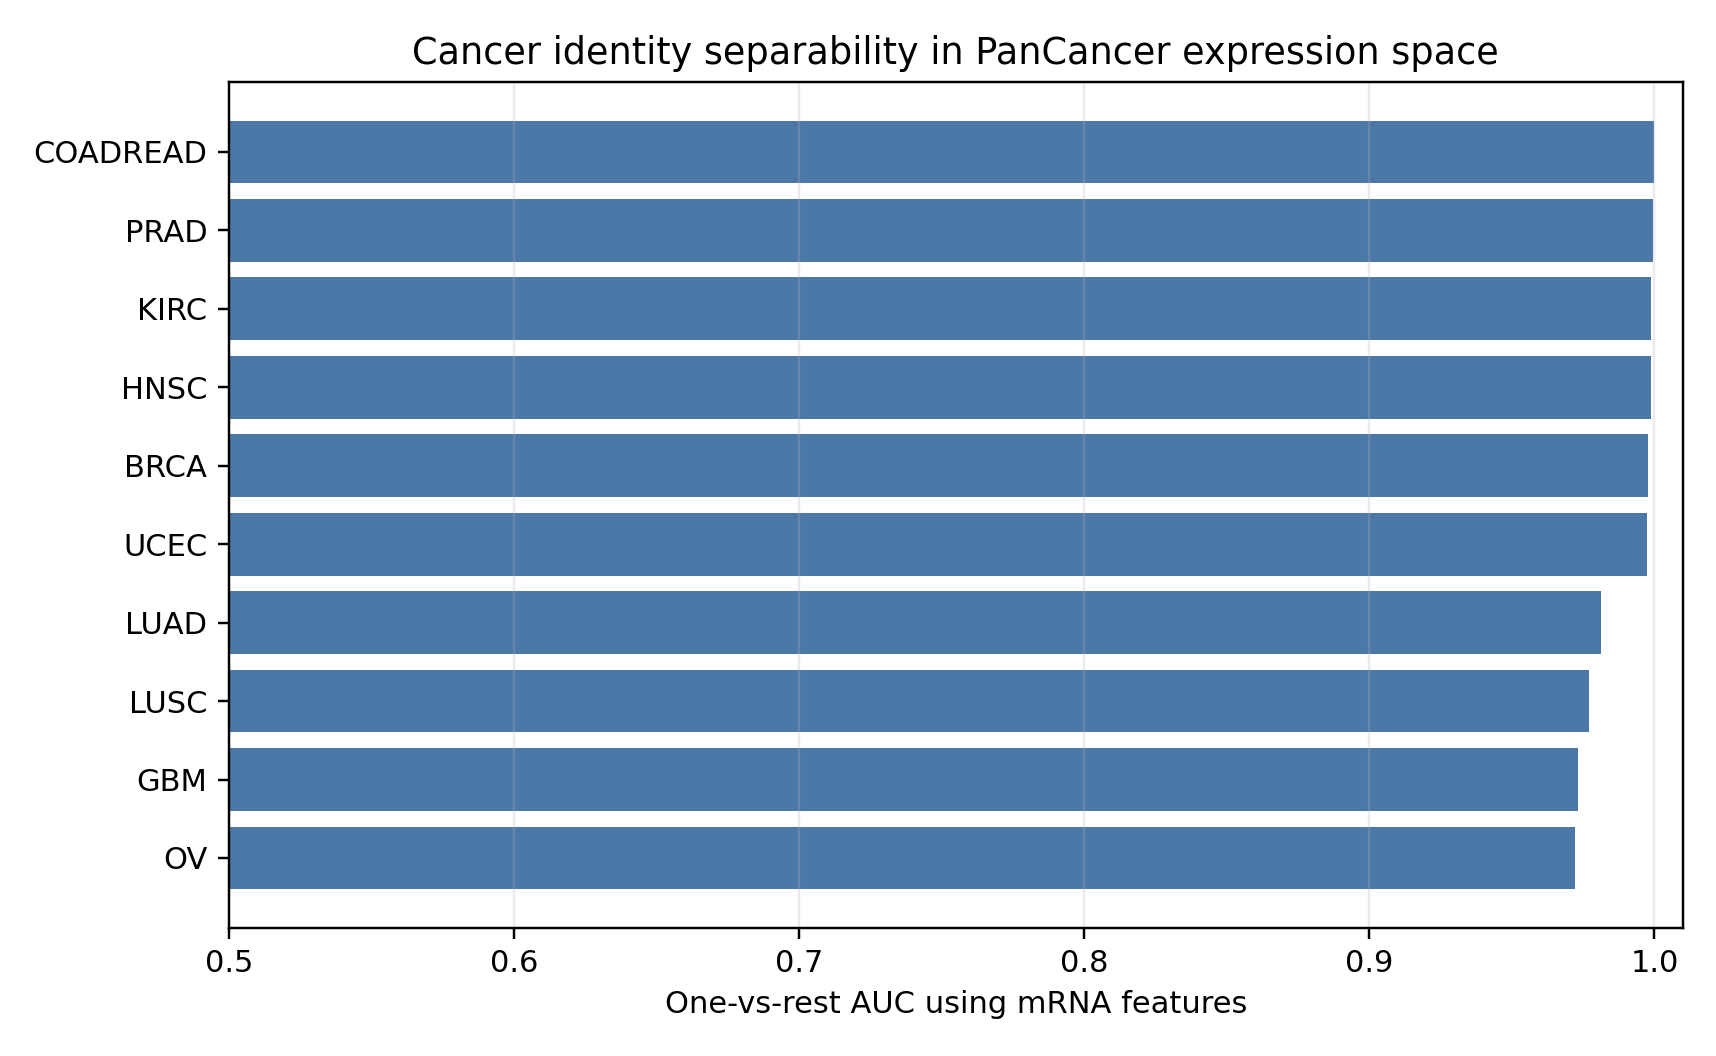
\includegraphics[width=0.86\textwidth]{figures/pancancer_cancer_separability_auc.png}
\caption{One-vs-rest cancer identity separability using mRNA features in the 10-cancer PanCancer table. All cancer types were highly separable from the rest, illustrating the strength of tissue/cancer identity signals in pan-cancer molecular data.}
\label{fig:cancer_sep}
\end{figure}

\begin{figure}[ht]
\centering
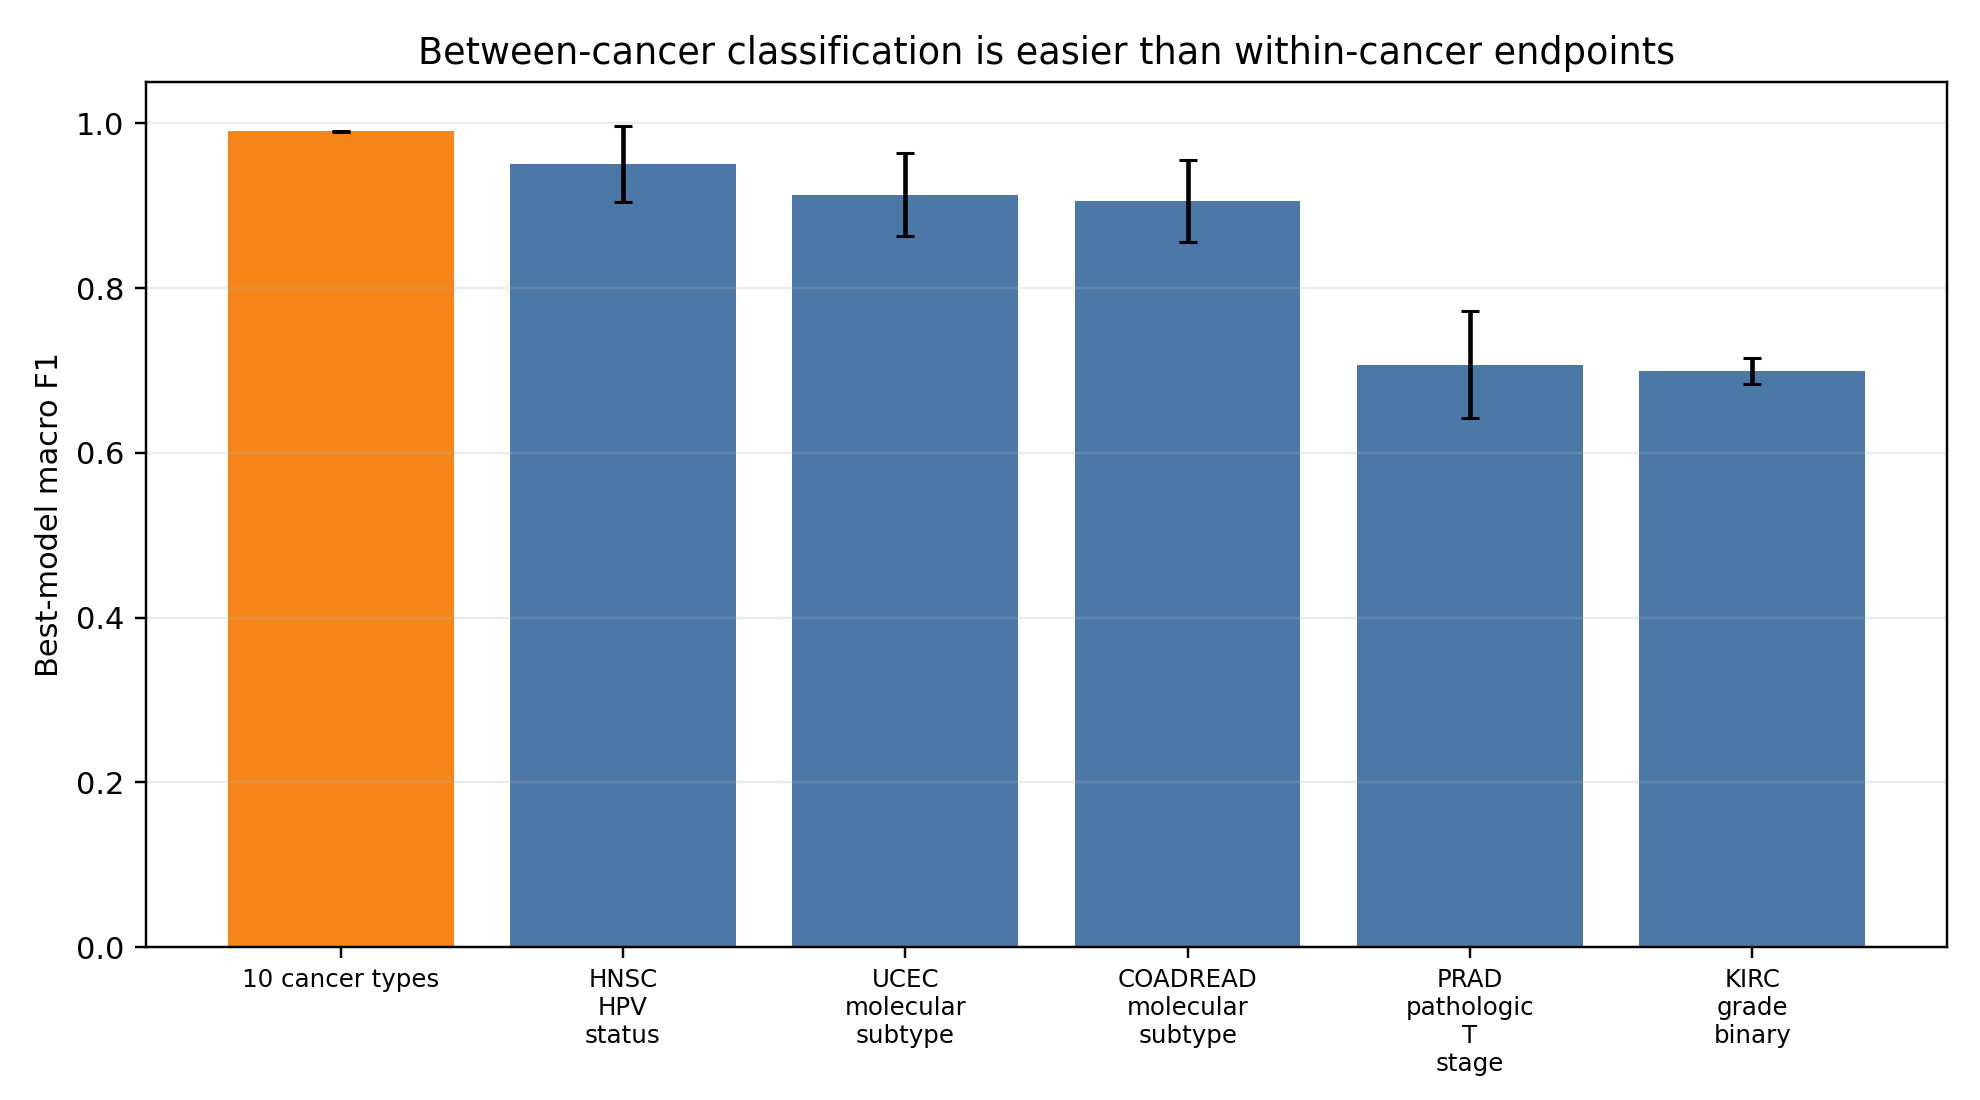
\includegraphics[width=\textwidth]{figures/pancancer_vs_internal_task_f1.png}
\caption{Best macro F1 for the 10-class PanCancer cancer-type task compared with five within-cancer endpoint tasks. The between-cancer task was substantially easier than the KIRC grade and PRAD pathologic T-stage tasks.}
\label{fig:task_difficulty}
\end{figure}

\subsection{The BRCA external-validation case study shows different shift profiles}

In the BRCA marker-expression case study, CPTAC 2020 was more separable from the TCGA/METABRIC source distribution than SMC 2018 or SCAN-B/GSE96058, with a domain separability AUC of 0.7596. SMC 2018 and SCAN-B/GSE96058 were close to random separability in this marker space (0.5165 and 0.5133, respectively). External macro F1 did not follow a simple monotonic relationship with separability: ExtraTrees performed best on SMC 2018, whereas logistic regression performed best on CPTAC 2020. These results suggest that cohort shift is not a single scalar obstacle; its effect depends on the model, label distribution, and external cohort structure.

\begin{figure}[ht]
\centering
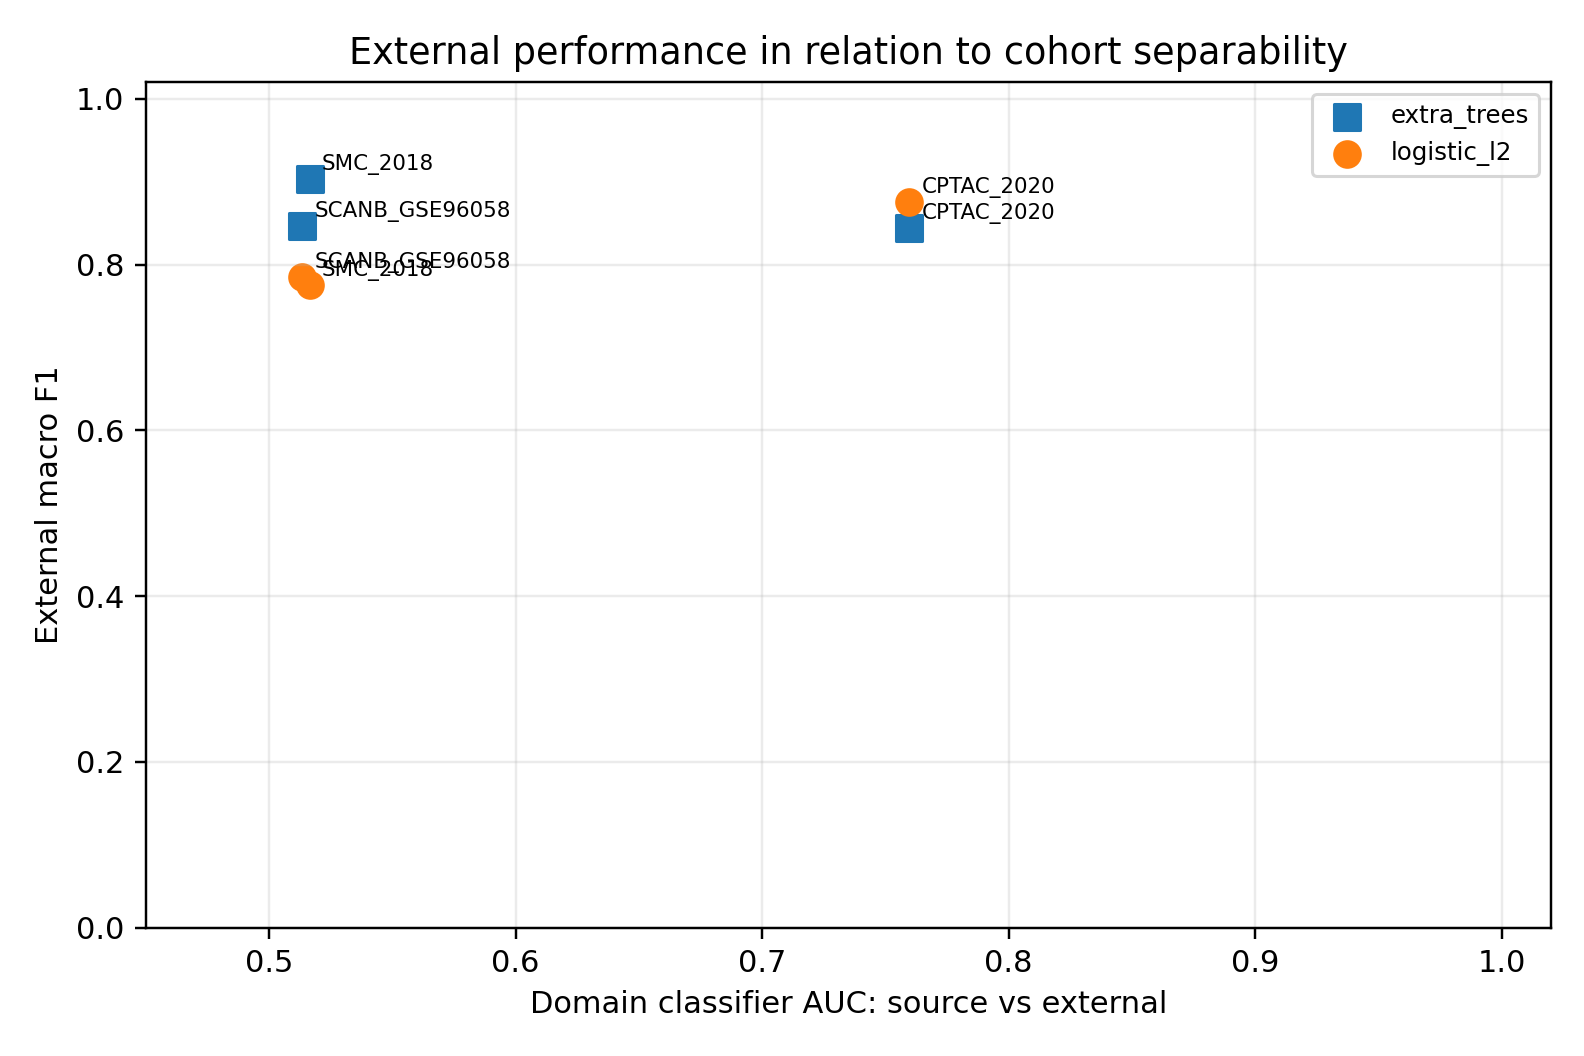
\includegraphics[width=0.86\textwidth]{figures/domain_shift_scatter.png}
\caption{BRCA external macro F1 in relation to source-versus-external cohort separability. The domain classifier AUC was computed in the 83-gene breast cancer marker expression space and transformed to separability AUC \(\max(AUC,1-AUC)\).}
\label{fig:domain_shift}
\end{figure}

\begin{table}[ht]
\centering
\caption{BRCA external-validation case study and domain-shift summary.}
\resizebox{\textwidth}{!}{%
\begin{tabular}{llrrrr}
\toprule
Dataset & Model & Macro F1 & Balanced accuracy & Mean standardized shift & Domain separability AUC \\
\midrule
CPTAC 2020 & ExtraTrees & 0.8440 & 0.8203 & 0.0384 & 0.7596 \\
SCAN-B/GSE96058 & ExtraTrees & 0.8465 & 0.8526 & 0.0381 & 0.5133 \\
SMC 2018 & ExtraTrees & 0.9028 & 0.9190 & 0.0652 & 0.5165 \\
TCGA/METABRIC validation & ExtraTrees & 0.8225 & 0.8016 & 0.0000 & 0.5000 \\
CPTAC 2020 & Logistic L2 & 0.8749 & 0.9013 & 0.0384 & 0.7596 \\
SCAN-B/GSE96058 & Logistic L2 & 0.7851 & 0.8603 & 0.0381 & 0.5133 \\
SMC 2018 & Logistic L2 & 0.7751 & 0.8732 & 0.0652 & 0.5165 \\
TCGA/METABRIC validation & Logistic L2 & 0.8219 & 0.8521 & 0.0000 & 0.5000 \\
\bottomrule
\end{tabular}
}
\label{tab:domain_shift}
\end{table}
